%!TeX program = xelatex
\documentclass[12pt,hyperref,a4paper,UTF8]{ctexart}
\usepackage{SHUreport}
\usepackage{subcaption}
\usepackage{graphicx}
\setcounter{secnumdepth}{5}
%%-------------------------------正文开始---------------------------%%
\begin{document}

%%-----------------------封面--------------------%%
\cover

%%------------------摘要-------------%%
%\begin{abstract}
%
%在此填写摘要内容
%
%\end{abstract}

\thispagestyle{empty} % 首页不显示页码

%%--------------------------目录页------------------------%%
\newpage
\tableofcontents

%%------------------------正文页从这里开始-------------------%
\newpage

%%可选择这里也放一个标题
%\begin{center}
%    \title{ \Huge \textbf{{标题}}}
%\end{center}

\section{任务需求分析}   

\subsection{问题}

以上述IR作为输入,我们提供基本的IR的parser,根据上述IR,完成调度、寄存器及操作的绑定、控制逻辑综合,函数输入的数组综合为SRAM存储器,需要根据load/store指令来读写存储器数据。最终生成RTL代码。基本计算操作可以调用RTL计算模块,或直接使用原始操作符。

\subsection{需求分析}

1. 实现寄存器的绑定和调度
2. 实现控制逻辑综合

\section{团队分工情况}

\subsection{分工情况}

\begin{table}[h]
    \centering
    \begin{tabular}{|c|c|c|}
    \hline
    \textbf{姓名} & \textbf{分工} \\ \hline
    秦振航 & 寄存器的绑定和操作调度\\ \hline
    杨远达 & 控制逻辑综合 \\ \hline
    \end{tabular}
\end{table}

\section{程序实现思路与数据结构}

\subsection{代码结构}

项目的源代码在HLS/src文件夹中,包含以下模块:

\begin{enumerate}
    \item Paser 输入文件解析模块。
    \item main 主函数。
    \item Basic 基础类,包括语法块,句子,以及调度绑定时需要的点类。
    \item HLSHandler 高层次综合的实现类
\end{enumerate}

\subsection{命令行参数解析}

-i 输入解析文件名

\subsection{实现思路}

整体上分为两个步骤,首先将解析后的文件进行寄存器的绑定和操作调度,然后根据调度结果进行控制逻辑综合。

\subsubsection{数据结构}

\paragraph{绑定和调度}

对于操作的调度和寄存器绑定而言,主要沿用Basic.hpp中的类,在function类下添加<变量,寄存器>的哈希表,以及全局变量$global\_regs$和常量$constant\_regs$。

在statement类下添加在该块逻辑里操作开始和结束的时间。

对于调度过程中,需要采用ASAP算法进行拓扑排序,所以引入一个节点类$point$,带有节点值,前序节点,后序节点等信息,用于进行拓扑排序。

\subsection{寄存器的绑定和操作调度}

首先,在分配寄存器之前需要将寄存器分为全局寄存器,局部寄存器和常量三类,对于全局寄存器,整个函数流程稳定分配一个寄存器,可以在程序开头就分配好,对于常量而言不需要寄存器直接赋值即可,对于局部寄存器需要在块内做左边算法来获得其生命周期和所指的变量。

对于常量,既不是函数输入,仅出现在右值的量。将其设置为寄存器-1。

对于全局变量,即在两个或以上的块出现的量,对于每一块设置一个$get\_vars$的方法,用于统计出现在本块中的所有变量,然后将块与块之间做交集,将交集求并即可得到全局变量表。在程序开始时依次分配寄存器。

对于局部变量,采取左边算法进行寄存器的动态绑定。需要首先建立拓扑排序树。对于一个block:

\begin{enumerate}
\item 依次取出Block中的statement,对于每个statement,将$var$建立节点放入树中。
\item 遍历操作数,查看是否已经在树中,如果在,则将$var$的入度加1,并将操作数对应节点的后置节点设为当前节点,当前节点前置节点设为操作数对应节点,如果不在,说明为常量或者全局变量,对入度没有影响。
\item 遍历$vector<point>points$,寻找入度为0的点,入队,设置开始时间为0,从寄存器数组$vector<color>colors$中取出一个颜色,如果寄存器数组为空,则新增一种颜色。
\item 如果队列不为空,循环,取出队首,将队首的后置节点入度减1,将颜色寄存器释放存。遍历队列中入度为0的点,更新点的开始时间,将颜色寄存器分配给该点,入队。
\item 队列为空,程序结束,遍历statement,设置statement的开始时间为$var$的开始时间。完成操作数的调度。
\end{enumerate}

\begin{figure}
    \centering
    \includegraphics[width=0.5\textwidth]{figures/binding\_result.png}
    \caption{拓扑排序树}
    \label{fig:完成调度后的结果}
\end{figure}
\section{测试方法和验证}

程序的输入数组a,b综合为ram,在vivador中进行仿真。
对于函数的输入,n为外界规定的数组长度,a[i],b[i]为从ram中读取的数值。
对于输出,cl对应输出结果result,需要结果标志信号done\_flag。在执行load指令时,需要制定地址i,即a\_ddr和b\_ddr,同时需要读使能信号a\_rd\_en和b\_rd\_en。

其外部完整电路为(详见top.v):

\begin{figure}[htbp]
    \centering
    \begin{minipage}{0.45\textwidth}
        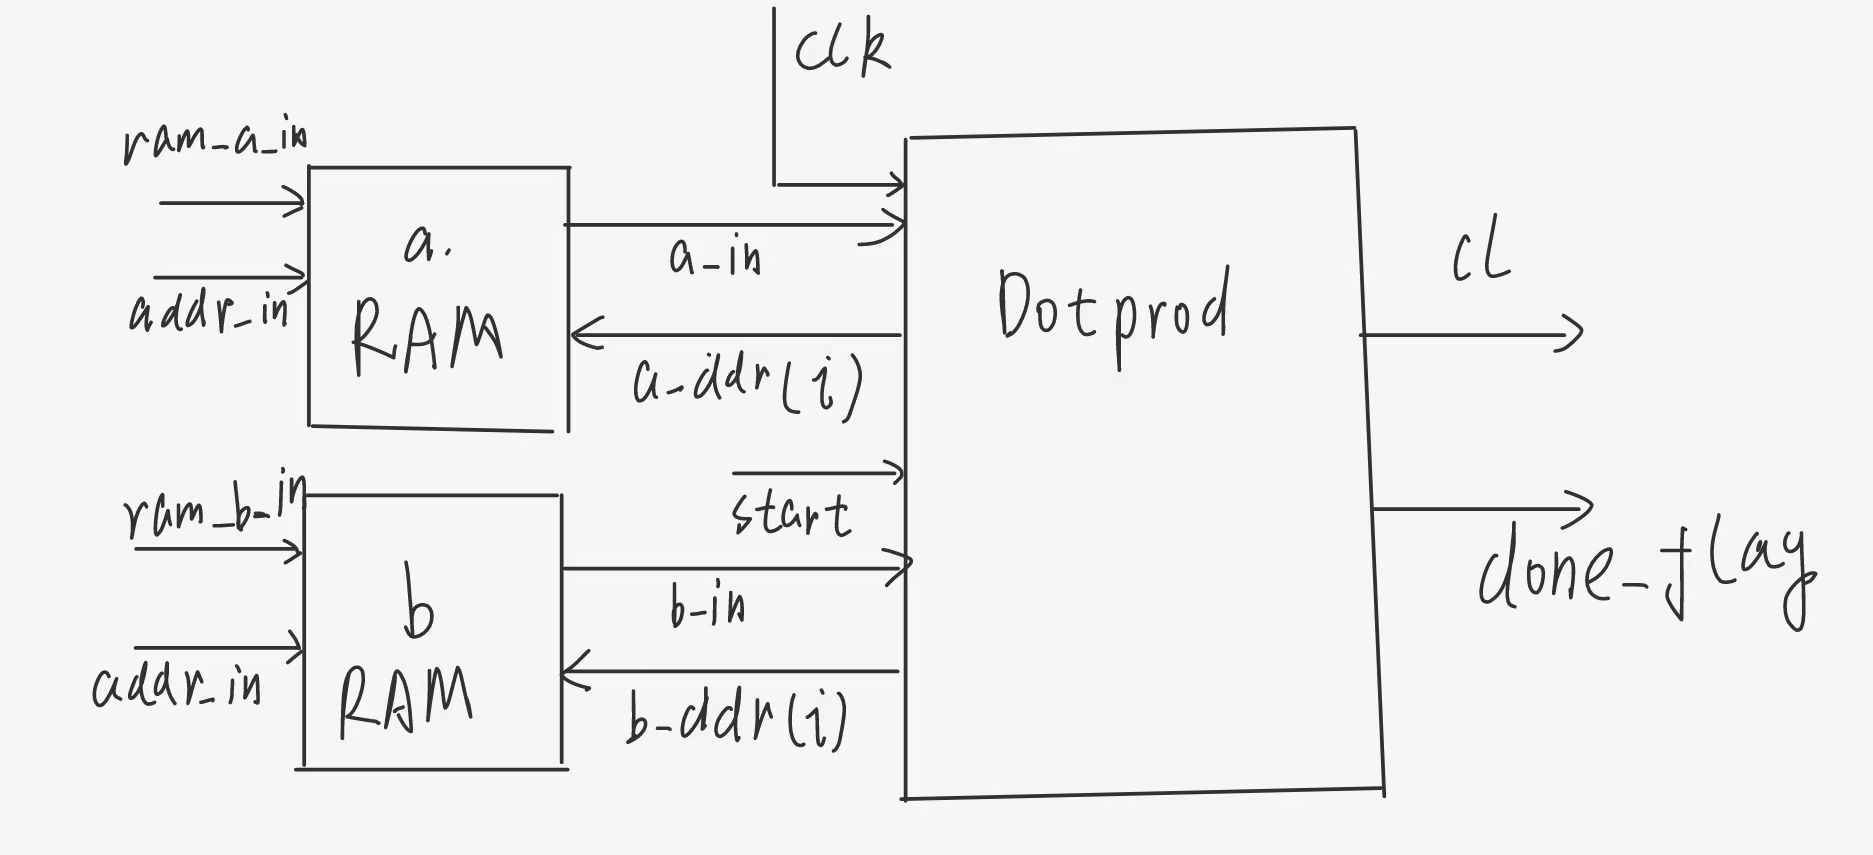
\includegraphics[width=\linewidth]{./figures/结构示意图.png}
        \caption{结构示意图}
        \label{fig:sub1}
    \end{minipage}
    \hfill % 添加适当的空间
    \begin{minipage}{0.45\textwidth}
        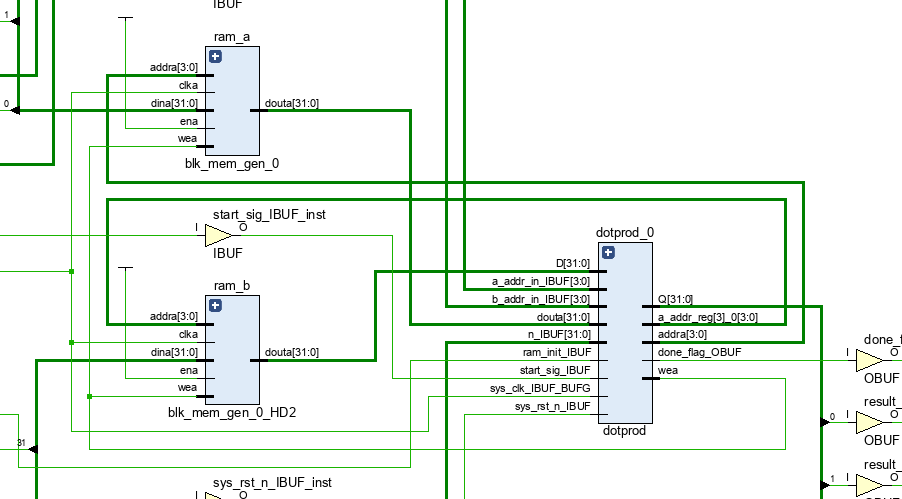
\includegraphics[width=\linewidth]{./figures/综合结果.png}
        \caption{综合结果}
        \label{fig:sub2}
    \end{minipage}
\end{figure}

\subsection{测试方法}

可知该IR的输入输出为数组,输出为数组点乘,通过测试文件tb_top.v,初始化给两个ram写入[0,9]十个数,然后复位生成电路,开始计算结果。

\subsection{验证结果}
输入后的结果如图,输入为从9到0十个数,最终输出为285(8'f11d)
\begin{figure}[htbp]
    \centering
    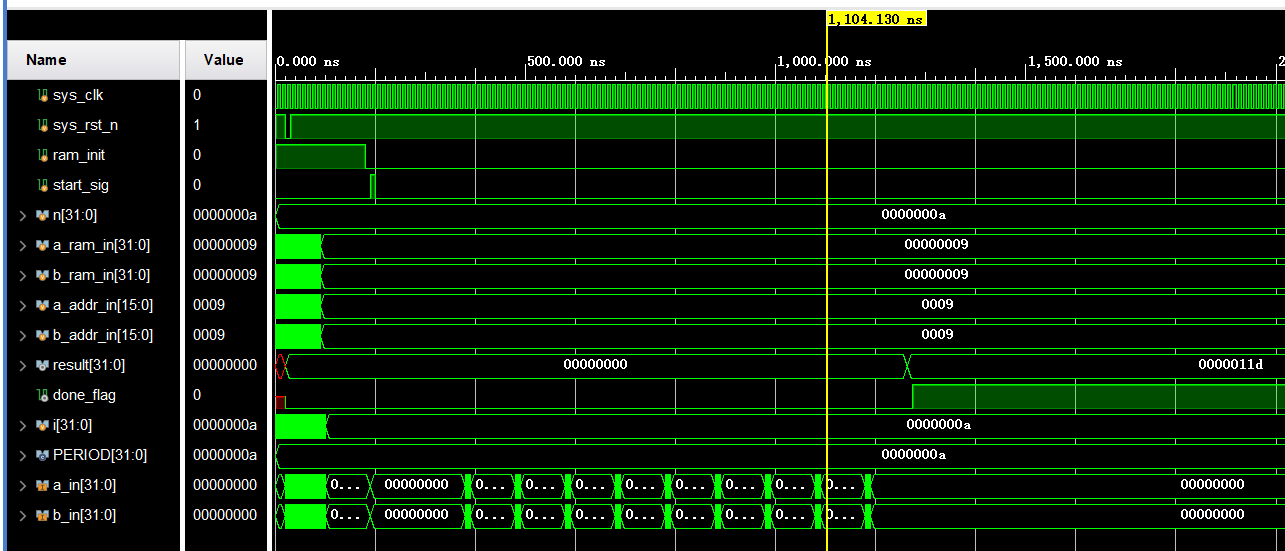
\includegraphics[width=0.5\textwidth]{figures/仿真结果.png}
    \caption{结果}
    \label{fig:仿真结果}
\end{figure}


\end{document}